\def\papertitle{On the design and use of once-differentiable high dynamic
resolution atoms for the Distribution Derivative Method}
\def\paperauthorA{Nicholas Esterer}
\def\paperauthorB{Philippe Depalle}
\documentclass[plainsections,landscape]{sciposter}


\usepackage{epsfig}
\usepackage{amsmath}
\usepackage{amssymb}
\usepackage{multicol}
\usepackage{tcolorbox}
%\usepackage{fancybullets}
%\usepackage{amsmath,amssymb,amsfonts,amsthm}
%\usepackage{euscript}
%\usepackage[latin1]{inputenc}
%\usepackage[T1]{fontenc}
%\usepackage{ifpdf}
%
%\usepackage[english]{babel}
%\usepackage{caption}
%\usepackage{subfig} % or can use subcaption package
%\usepackage{color}
%\usepackage{cite}
%\usepackage{float}
%
%\usepackage{hyphenat}
%\hyphenation{spher-oidal}
%%\hyphenation{amp-li-tude}
%%\hyphenation{mod-u-lat-ed}
%
%\usepackage{times}

\newtheorem{Def}{Definition}

%\definecolor{BoxCol}{rgb}{0.9,0.9,0.9}
% uncomment for grey background to \section boxes 
% for use with default option boxedsections

%\definecolor{BoxCol}{rgb}{0.9,0.9,1}
% uncomment for light blue background to \section boxes 
% for use with default option boxedsections

%\definecolor{SectionCol}{rgb}{0,0,0.5}
% uncomment for dark blue \section text 

% Flowchart drawing stuff
\usepackage{tikz}
\usetikzlibrary{shapes.geometric, arrows, positioning, calc}
\tikzstyle{startstop} = [rectangle,draw=black,text centered]%, rounded corners, minimum width=3cm, minimum height=1cm,text centered, draw=black, fill=red!30]
\tikzstyle{io} = [trapezium, trapezium left angle=70, trapezium right angle=110, minimum width=3cm, minimum height=1cm, text centered, draw=black, fill=blue!30]
\tikzstyle{process} = [rectangle, minimum width=3cm, minimum height=0cm, text
centered, draw=black, text width=0.3\columnwidth]
\tikzstyle{emptybox} = []
\tikzstyle{decision} = [diamond, minimum width=3cm, minimum height=1cm, text centered, draw=black, fill=green!30]
\tikzstyle{arrow} = [thick,->,>=stealth]
\tikzstyle{noarrow} = [thick,-,>=stealth]

\title{\papertitle}

% Note: only give author names, not institute
\author{\paperauthorA{} and \paperauthorB{}}
 
% insert correct institute name
\institute{Sound Processing and Control Laboratory (SPCL) at McGill University}

\email{nicholas.esterer@mail.mcgill.ca, philippe.depalle@mcgill.ca}  % shows author email address below institute

\input{ddm_snr_win_comp_defs.txt}
\input{comp_offset_chirp_est_err_defs.txt}

\begin{document}
%define conference poster is presented at (appears as footer)

\conference{{\em{\small{The 20$^{\text{\itshape th}}$ International Conference on Digital Audio Effects (DAFx-17), Edinburgh, UK, September 5--9, 2017}}}}

%\LEFTSIDEfootlogo  
% Uncomment to put footer logo on left side, and 
% conference name on right side of footer

% Some examples of caption control (remove % to check result)

%\renewcommand{\algorithmname}{Algoritme} % for Dutch

%\renewcommand{\mastercapstartstyle}[1]{\textit{\textbf{#1}}}
%\renewcommand{\algcapstartstyle}[1]{\textsc{\textbf{#1}}}
%\renewcommand{\algcapbodystyle}{\bfseries}
%\renewcommand{\thealgorithm}{\Roman{algorithm}}

\maketitle

%%% Begin of Multicols-Enviroment
\setlength{\columnseprule}{0pt}
\begin{multicols}{3}

%%% Abstract
\begin{abstract}
    The accuracy of the Distribution Derivative Method (DDM)
    \cite{betser2009sinusoidal} is evaluated on mixtures of chirp signals. It is
    shown that accurate estimation can be obtained when the sets of atoms for
    which the inner product is large are disjoint.  This amounts to designing
    atoms with windows whose Fourier transform exhibits low sidelobes but which
    are once-differentiable in the time-domain. A technique for designing
    once-differentiable approximations to windows is presented and the accuracy
    of these windows in estimating the parameters of sinusoidal chirps in
    mixture is evaluated.
\end{abstract}

%%% Introduction
\section{Introduction}
\label{sec:intro}

Recently, there has
been interest in using higher-order phase functions for the argument of sinusoidal
    functions \cite{xuepiecewise} as the estimation of
their parameters has been made possible by a set of techniques 
using signal derivatives \cite{hamilton2012unified}.

For comparison with previous research on the DDM, we consider the estimation -- via the DDM -- of the parameters of a
    parabolic phase function for which the imaginary parts of the parameters
    represent the initial phase, frequency and frequency slope. The real parts
    of the parameters represent the initial amplitude, amplitude slope and
    amplitude curvature.

The DDM requires a set of atoms that are once-differentiable everywhere in
    the time-domain from which the parameters are estimated. We
    show that on a mixture of sinusoids, accurate estimation for each sinusoid
    can be obtained under a single-component
assumption when components have roughly disjoint sets of atoms for which their
inner products take on large values. 

Encouraging disjointedness amounts to designing atoms whose Fourier
    transform exhibits low side-lobes under the additional constraint that
    the atoms be everywhere once-differentiable. We show how to design atoms
    with this latter property based on the shapes of ideal windows.

\section{Estimating the \lowercase{$a_{p,q}$} of $P$ components}
\begin{tcolorbox}
    \begin{multicols}{2}
The model for signal $x$ is
%
\begin{equation}
    x(t) = \sum_{p=1}^{P} x_{p}(t) + \eta(t)
\end{equation}
%
with
%
\begin{equation}
    \label{eq:polyphaseexpmix}
    x_{p}(t) = \exp(a_{p,0} + \sum_{q=1}^{Q} a_{p,q} t^q)
\end{equation}
%
and $\eta$ Gaussian-distributed white noise. 
    \end{multicols}
\end{tcolorbox}

\begin{tcolorbox}
\begin{multicols}{2}
Applying the DDM to a mixture of $P$ componentes, we obtain%
\footnote{
$\mathcal{T}^{\alpha} : (\mathcal{T}^{\alpha}x)(t) = t^{\alpha}x(t)$

$\left\langle x , \psi \right\rangle = 
\int_{-\infty}^{\infty}x(t)\overline{\psi}(t)dt$
}
%
\begin{multline}
    \label{eq:mixest}
    \sum_{p=1}^{P} \left(
    \sum_{q=1}^{Q} q a_{p,q} 
    \left\langle \mathcal{T}^{q-1} x_{p} , \overline{\psi} \right\rangle
    + \left\langle x_{p}, \frac{d\overline{\psi}}{dt} \right\rangle \right)
    \\
    = 0
\end{multline}
%
From this we see if $\left\langle \mathcal{T}^{q-1} x_{p} , \overline{\psi}_{r}
\right\rangle$ and $\left\langle x_{p}, \frac{d\overline{\psi_{r}}}{dt} \right\rangle$
are small for all but $p = p^{\ast}$ and a subset of $R$ atoms\footnote{%
The notation $x^{\ast}$ will mean the value of the argument $x$ maximizing or minimizing some
function.
}%
, we can simply estimate the parameters $a_{p^{\ast},q}$ using
\begin{equation}
    \sum_{q=1}^{Q} q a_{{p^{\ast}},q} 
    \left\langle \mathcal{T}^{q-1} x_{p^{\ast}} , \overline{\psi}_{r} \right\rangle
    = -\left\langle x_{p^{\ast}}, \frac{d\overline{\psi}_{r}}{dn} \right\rangle
\end{equation}
for $1 \leq r \leq R$.
\end{multicols}
\end{tcolorbox}

\begin{tcolorbox}
\begin{multicols}{2}
To compute $a_{p^{\ast},0}$ we define
\begin{equation}
    \gamma_{p^{\ast}}(t) = \exp \left( \sum_{q=1}^{Q} a_{p^{\ast},q} t^{q} \right)
\end{equation}
and estimate $a_0$ as
\begin{equation}
    \label{eq:ddmesta0}
    a_0 = \log \left( \left\langle x , \gamma \right\rangle \right)
        - \log \left( \left\langle \gamma , \gamma \right\rangle \right)
\end{equation}
\end{multicols}
\end{tcolorbox}

\section{Designing the $\psi_{r}$}
\label{sec:designingatoms}
\begin{tcolorbox}
\begin{multicols}{2}
%
Canonically, the chosen atoms $\psi_{\omega}(t)$ 
are the products of the elements of the Fourier basis and an appropriately
chosen window $w$ that is once differentiable and finite, i.e.,
%
\begin{equation}
    \label{eq:fourieratom}
    \psi_{\omega}(t) = w(t) \exp(-j \omega t)
\end{equation}
%
Defining $N = \frac{L_{t}}{T}$ and angular frequency at bin $r$ as $\omega_{r} = 2
\pi \frac{r}{N}$, the approximate inner product is then
%
\begin{equation}
    \label{eq:approxinnerprod}
    \left\langle x , \psi_{\omega} \right\rangle \approx 
    \sum_{n=0}^{N-1} x(Tn) w(Tn) \exp(-2 \pi j r \frac{n}{N}) 
\end{equation}
%
i.e., the definition of the DFT of a windowed signal.
Therefore choosing $\psi$ amounts to a
Fourier window design problem minimizing its side-lobes, under the constraint
that the window be differentiable in $t$ and finite.
\end{multicols}
\end{tcolorbox}

\section{Differentiable approximations to windows}
%
\newcommand{\imsize}{\columnwidth}
\begin{figure}
\begin{center}
    {\resizebox{\imsize}{!}{\includegraphics{{search_dpw_bw_m}.eps}}}
\end{center}
\caption{\label{fig:dpw} Comparing the main-lobe and asymptotic power
spectrum characteristics of the continuous 4-term Nuttall window, the digital
prolate window with $W=0.008$, and the continuous approximation to the digital
prolate window.}
\end{figure}
%

\begin{tcolorbox}
\begin{multicols}{2}
A differentiable approximation to a symmetrical window can be designed in a
straightforward way. In \cite{harris1978use} and \cite{rabiner1970approach} it
is shown how to design optimal windows of length $N$ samples using a linear
combination of $M$ harmonically related cosines
\begin{equation}
    \tilde{w}(n) = \sum_{m=0}^{M-1} b_{m} \cos (2 \pi m \frac{n}{N})
\mathcal{R}(\frac{n}{N})
\end{equation}
where $\mathcal{R}$ is the \textit{rectangle function}. This function is
discontinuous
at $n = \frac{\pm N}{2}$, and therefore not differentiable there, unless
$\sum_{m=0}^{M-1} b_{m} \cos ( \pm \pi m ) = 0$.

Therefore, we choose the $b_{m}$ so that
the window $\tilde{w}$'s squared approximation error to $w$ is minimized while having
$\tilde{w}(\frac{\pm N}{2}) = 0$, i.e. we find the solution $\{ b^{\ast}_{m} \}$ to the
mathematical program
\begin{equation}
    \label{eq:searchcontwinprogram}
    \text{minimize}
    \sum_{n=0}^{N-1} ( w(n) 
        - \sum_{m=0}^{M-1} b_{m} \cos(2 \pi m \frac{n}{N}))^{2}
\end{equation}
\begin{equation}
    \text{subject to} \\
    \sum_{m=0}^{M-1} b_{m} \cos(\pi m ) = 0
\end{equation}
which can be solved using constrained least-squares\cite[p.~585]{golub1996matrix}.
\end{multicols}
\end{tcolorbox}

\begin{tcolorbox}
\begin{multicols}{2}
Using this technique, we designed a continuous approximation to a digital prolate
spheroidal window of length $N=512$ and $W=0.008$. The coefficients
are described in Table~\ref{tab:contprolate} and a comparison with other
windows is shown in Figure~\ref{fig:dpw}.

\begin{table}[]
    \caption{The coefficients of the once-differentiable approximation to a digital prolate
    window.
    \label{tab:contprolate}}
    \begin{center}
        \begin{tabular}{c c c}
            $b_0$ & $ = $ & 3.128 $\times 10^{-1}$ \\
            $b_1$ & $ = $ & 4.655 $\times 10^{-1}$ \\
            $b_2$ & $ = $ & 1.851 $\times 10^{-1}$ \\
            $b_3$ & $ = $ & 3.446 $\times 10^{-2}$ \\
            $b_4$ & $ = $ & 2.071 $\times 10^{-3}$ 
        \end{tabular}
    \end{center}
\end{table}%
\end{multicols}
\end{tcolorbox}

\section{The performance of improved windows on signals with 2 components}

To investigate the performance of the various windows when estimating the
parameters of components in mixture we synthesized signals using
Eq.~\ref{eq:polyphaseexpmix} with $P=2$ and $Q=2$ and parameters chosen from the
uniform distributions specified in \cite{betser2009sinusoidal} and evaluated
the parameter estimation accuracy at various differences between local maxima in
the mixture's power-spectrum. The procedure is
summarized in Fig.~\ref{fig:2cevalflowchart}.

$d$ was incremented by $\Delta_{d} = \Dstep{}$ and so
$\hat{d}$ was not generally integral valued in this case.

\begin{figure}
    \centering
            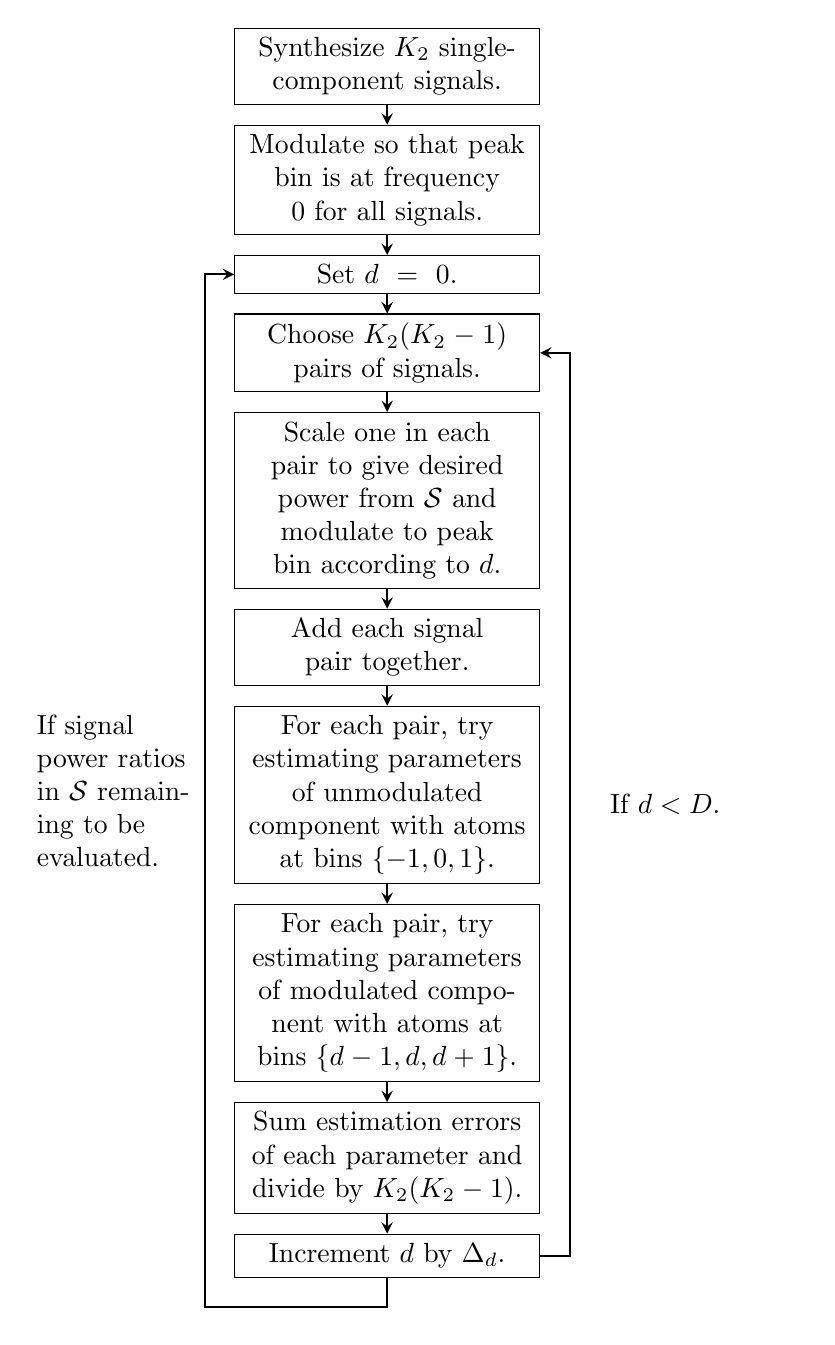
\begin{tikzpicture}[node distance=0.25cm]
                \node (start) [process] at (0,0) {Synthesize $K_{2}$
                single-component signals.};
                \node (modulate) [process, below = of start] {Modulate so that
                peak bin is at frequency 0 for all signals.};
                \node (setd) [process, below = of modulate] {Set $d=0$.};
                \node (choosepair) [process, below = of setd] {Choose
                    $K_{2}(K_{2}-1)$ pairs of signals.};
                \node (dum1) [emptybox, right = of choosepair] {};
                \node (scaleone) [process, below = of choosepair] {Scale one in
                each pair to give desired power from $\mathcal{S}$ and modulate to peak bin
                according to $d$.};
                \node (addpair) [process, below = of scaleone] {Add each signal
                pair together.};
                \node (tryestimate1) [process, below = of addpair] {For each
                pair, try
                estimating parameters of unmodulated component with atoms at
                bins $\{-1,0,1\}$.};
                \node (tryestimate2) [process, below = of tryestimate1] {For
                each pair, try
                estimating parameters of modulated component with atoms at bins
                $\{d-1,d,d+1\}$.};
                \node (sumerrs) [process, below = of tryestimate2] {Sum estimation errors of
                each parameter and divide by $K_{2}(K_{2}-1)$.};
                \node (incd) [process, below = of sumerrs] {Increment $d$ by
                $\Delta_{d}$.};
                \node (dum2) [emptybox, right = of incd] {};
                \node (dum3) [emptybox, below = of incd] {};
                \node (dum3b) [emptybox, left = of incd] {};
                \node (dum4) [emptybox] at (dum3b |- dum3) {};
%                \node let \p{dum3b}=(dum3b), \p{dum3}=(dum3) in (dum4) [emptybox] at (\x{dum3b},\y{dum3}) {};
                \node (dum5) [emptybox, left = of setd] {};

                \draw [arrow] (start) -- (modulate);
                \draw [arrow] (modulate) -- (setd);
                \draw [arrow] (setd) -- (choosepair);
                \draw [arrow] (choosepair) -- (scaleone);
                \draw [arrow] (scaleone) -- (addpair);
                \draw [arrow] (addpair) -- (tryestimate1);
                \draw [arrow] (tryestimate1) -- (tryestimate2);
                \draw [arrow] (tryestimate2) -- (sumerrs);
                \draw [arrow] (sumerrs) -- (incd);

                \draw [arrow] (incd) -- (dum2.center) -- (dum2.center) -- 
                    node [anchor=west,text width=2cm,minimum width=3cm] {If $d <
                    D$.} (dum1.center) 
                    -- (dum1.center) -- (choosepair);

                \draw [arrow] (incd) -- (dum3.center) -- (dum3.center) --
                (dum4.center) -- (dum4.center) -- 
                node [anchor=east,text width=2cm,minimum width=2cm]
                {If signal power ratios in $\mathcal{S}$ remaining to be
                evaluated.} (dum5.center) --
                 (dum5.center) -- (setd);

            \end{tikzpicture}
    \caption{The evaluation procedure for 2-component
    signals.\label{fig:2cevalflowchart}}
\end{figure}

\section{Acknowledgments}
This work was partially supported by grant from the Natural Sciences and Engineering Research Council of Canada awarded to Philippe Depalle (RGPIN-262808-2012).
\bibliographystyle{IEEEbib}
\bibliography{dafx-poster} % requires file DAFx17_tmpl.bib
\end{multicols}

\end{document}

